% !TeX root = ../main.tex
\section{V3：有限任务范围内的语义驱动工具组合}
\label{sec:v3}
\subsection{研究思路}
V3 将研究对象从固定计算链扩展到自然语言交互与工具组合。系统在已定义的科学能力范围内解释需求，建立结构化请求，并通过组合工具完成单点、优化、频率和派生量分析。相较 V2，其重点从过程保存转向用户语义与可执行操作之间的连接。

这一思路将科学求解能力主要保留在既有工具中，模型参与语义规范化、结果回答和有限修复。因而，V3 的评价既需验证基础工具的科学输出，也需考察对话情境中的条件修改、已有结果查询、澄清、拒绝与失败恢复。两类评价应区分统计。

\subsection{固定科学矩阵}
Scientific Matrix v1 在 5 类任务与 6 个分子对象中显式选择 11 个单元，11/11 单元通过，实际 ORCA 为 16 次、模型调用为 0，整体经过时间为 421.516 s。该矩阵采用固定请求和计划，检验组合执行与科学检查，不作为模型驱动端到端能力的证据。覆盖范围和部分科学结果见图 \ref{fig:v3-matrix}、表 \ref{tab:v3-science}。

\begin{figure}[htbp]
\centering
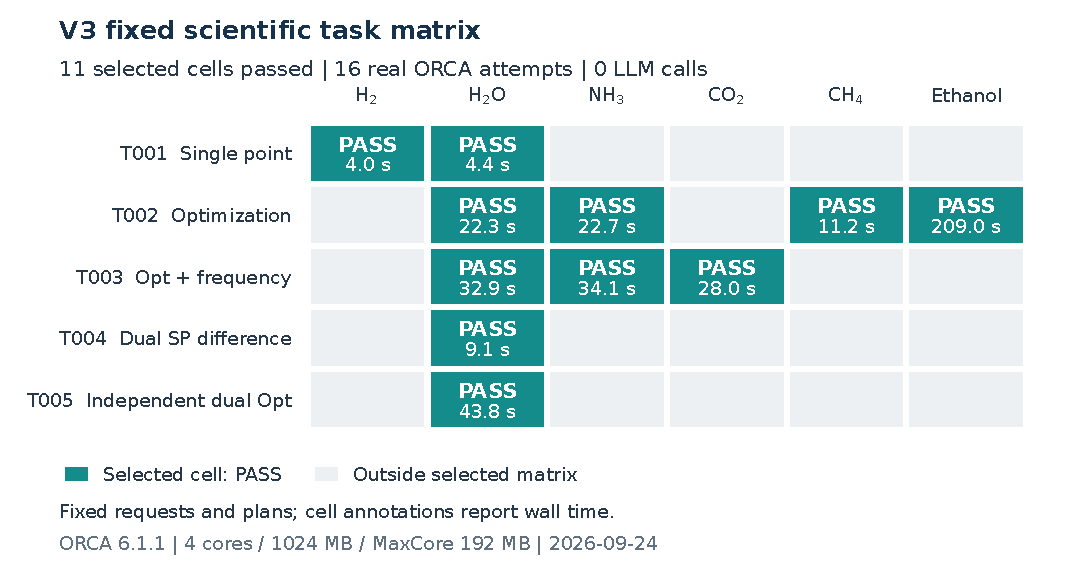
\includegraphics[width=\linewidth]{v3-scientific-matrix.pdf}
\caption{V3 固定科学矩阵。11 个启用单元全部通过，灰格未纳入评价分母。单元内标注经过时间；该批次使用真实 ORCA，模型调用为 0。}
\label{fig:v3-matrix}
\end{figure}

\begin{table}[htbp]
\centering\small
\caption{V3 科学矩阵的优化与频率结果。理论水平为气相 r$^{2}$SCAN-3c、零电荷、单重态，资源为 4 核、1024 MB、MaxCore 192 MB/进程。}
\label{tab:v3-science}
\begin{tabularx}{\linewidth}{p{1.8cm}rp{4.6cm}Y}
\toprule
分子 & 优化周期 & 最终优化电子能 / $\Eh$ & 相应频率检查\\
\midrule
H$_2$O & 5 & $-76.418938720985$ & 3 个正模式，局部极小值支持\\
NH$_3$ & 5 & $-56.541874067217$ & 6 个正模式，局部极小值支持\\
CO$_2$ & 3 & $-188.570062871358$ & 4 个正模式，局部极小值支持\\
CH$_4$ & 2 & $-40.494915367074$ & 仅优化，未作频率结论\\
乙醇 & 36 & $-155.002354316872$ & 仅优化，未作频率结论\\
\bottomrule
\end{tabularx}
\end{table}

水的三个正振动频率为 1653.24、3813.59、3932.75 cm$^{-1}$；CO$_2$ 为 668.14、668.14、1362.20、2422.54 cm$^{-1}$。线性 CO$_2$ 的五个外部零模式与四个振动模式被分别检查。两次固定矩阵记录的对照中，13 个电子能结果在输出的 12 位小数精度上相同，三套频率一致。这支持指定输入和设置下的数值重复性，不替代外部准确度评价。

\subsection{模型参与的核心基准}
Benchmark 1.2 core 的最终评分为 18/18，其分母包括 11 个固定科学题、5 个脚本化对话情境和 2 个名称解析题。16 项实际涉及计算，另两项为澄清与拒绝。实验驱动发送预定义话语，并在公开确认状态发送确认回复，经系统的正常对话入口执行，没有直接注入规范请求或计划。

该批次使用 DeepSeek Flash，共 37 次模型调用：语义规范化 19 次、结果回答 17 次、修复 1 次；专门 Intake/Planner 模型调用均为 0。输入、输出和总 tokens 分别为 140,953、6,985 和 147,938，整体经过时间为 667.547 s。ORCA 共尝试 23 次，包括 22 次成功和 1 次预设受控失败，随后执行一次有界修复。图 \ref{fig:v3-cost} 给出调用与耗时分布。

\begin{figure}[htbp]
\centering
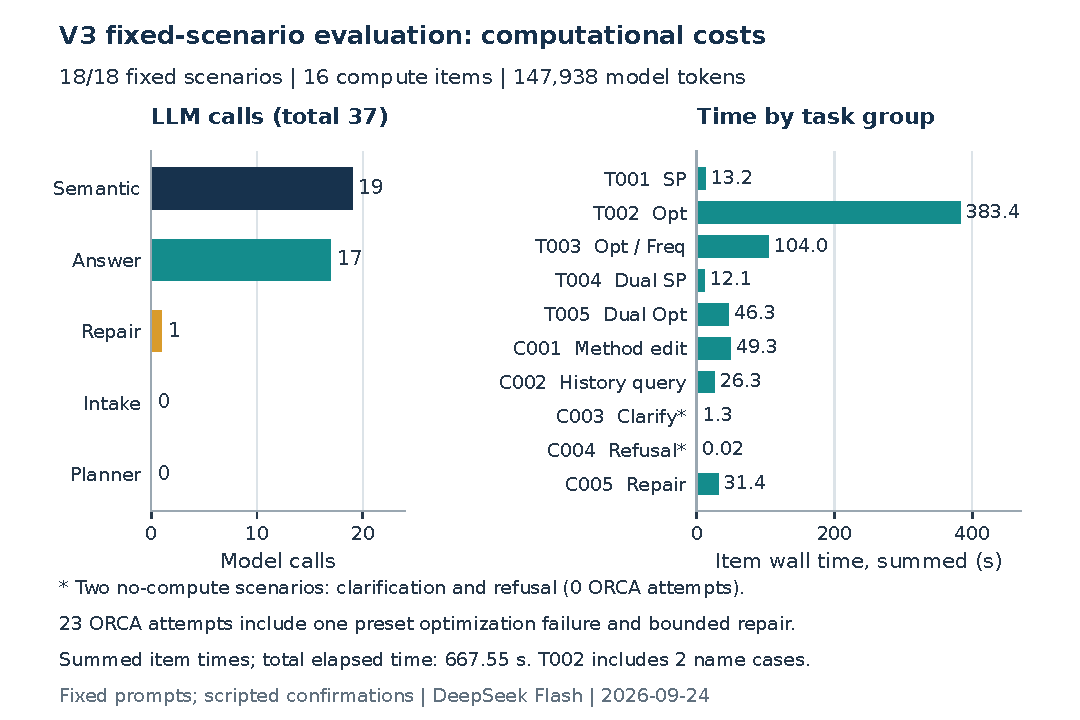
\includegraphics[width=\linewidth]{v3-core-costs.pdf}
\caption{V3 核心基准的模型调用分工与任务组耗时。18/18 表示预定义情境的最终评分，其中两项不执行计算；23 次 ORCA 尝试包含一次预设失败及其后续修复。各组的对象和步骤数不同，耗时不作效率排序。}
\label{fig:v3-cost}
\end{figure}

受控失败通过限制优化迭代次数产生，用于检验已定义修复路径，不能解释为自然故障发生率。最终评分还对一项确定性拒绝情境作过规则校准，保存观察没有重跑。因此，18/18 应理解为有限范围内的情境评分，而非任意自然语言任务的自主成功概率。

\subsection{方法边界与 V4 的研究动机}
V3 说明，自然语言语义、工具执行和有界修复可以在有限任务集合中协同运行。然而，科学题的方法、结构和目标受到预定义条件约束，对话也由脚本组织；完整扩展集与未见任务集未运行，数值结果未相对外部高精度参照评价。这些限制使现有成果主要支持已定义范围内的组合能力。

在此基础上，新的问题是：当科学需求要求已有工具未封装的采样、分析或算法时，是否必须由开发者增加专用求解模块？本文据此将 V4 的研究重点转向任务算法的现场生成，通过固定通用工具与生成代码的组合拓展任务表达，同时保持执行边界和科学验证要求。该过渡是基于已有证据的研究问题重构，不构成版本性能提升的预先结论。
